\documentclass{beamer}
\usepackage{luatexja-fontspec}
\setmainjfont[BoldFont=YuKyo_Yoko-Bold]{YuKyo_Yoko-Medium}
\setsansjfont[BoldFont=YuGo-Bold]{YuGo-Medium}
\usepackage{newpxtext,newpxmath}
\usepackage{graphicx}
\usepackage{minted}
\usepackage{hyperref}
\usetheme{Luebeck}
\usecolortheme{seahorse}
\usefonttheme{structurebold,serif}
\setbeamertemplate{navigation symbols}{\usebeamerfont{footline}\insertframenumber/\inserttotalframenumber}

\title{ルービックキューブ群をSageMathで見る}
\author{宇佐見 公輔}
\date{2020年10月31日}
\begin{document}
\maketitle

\begin{frame}
    \frametitle{自己紹介}

    職業:プログラマ / 趣味:数学

    \bigskip

    最近の活動:
    \begin{itemize}
        \item イジング模型(10月 / MathWills)
        \item ルービックキューブと群論(10月 / 関西日曜数学友の会)
        \item 平面の敷き詰めとルート系(6月 / 日曜数学会)
        \item 四元数のはなし(5月 / 関西日曜数学友の会)
    \end{itemize}
\end{frame}

\begin{frame}
    \frametitle{今回の内容}

    ルービックキューブは群論の言葉で考察することができます。

    \begin{figure}
        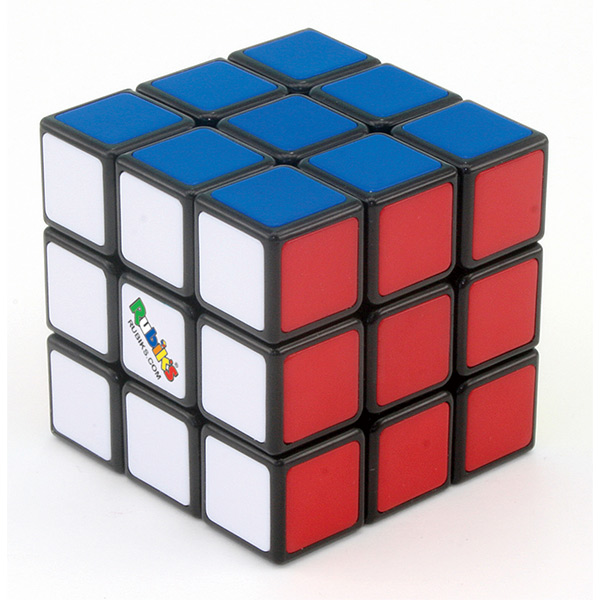
\includegraphics[scale=0.15]{images/rubik3.jpg}
    \end{figure}

    SageMathでルービックキューブ群について調べて遊んでみたいと思います。

    \begin{figure}
        
\includegraphics[scale=0.2]{images/logo_sagemath+icon_oldstyle.png}
    \end{figure}
\end{frame}

\begin{frame}
    \frametitle{ルービックキューブ考察にあたっての前提}

    3次元空間の中でキューブの位置や向きを固定します。キューブそのものを回転させることは考えません。

    キューブの操作は、各面を時計回りまたは反時計回りに90度ずつ動かすことを考えます。真ん中の列を回転させることはしません。

    \begin{figure}
        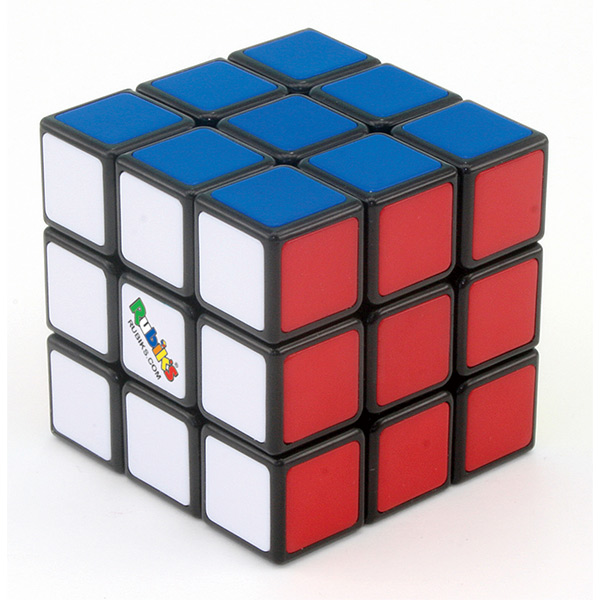
\includegraphics[scale=0.2]{images/rubik3.jpg}
    \end{figure}
\end{frame}

\begin{frame}
    \frametitle{小方体(cubelet)}

    \begin{itemize}
        \item 小方体:キューブを構成する小立方体。中心を除いて26個。
        \item 1面体:1つの面が外側に見えている小方体。6個。
        \item 2面体:2つの面が外側に見えている小方体。12個。
        \item 3面体:3つの面が外側に見えている小方体。8個。
    \end{itemize}

    \bigskip

    先ほどの前提から、1面体は動きません。2面体と3面体がキューブの操作によって移動します。
\end{frame}

\begin{frame}
    \frametitle{小面(facet)}

    キューブの各面を構成する正方形を小面と呼びます。各面で中央を除いて8個、全体で48個あります。

    \begin{figure}
        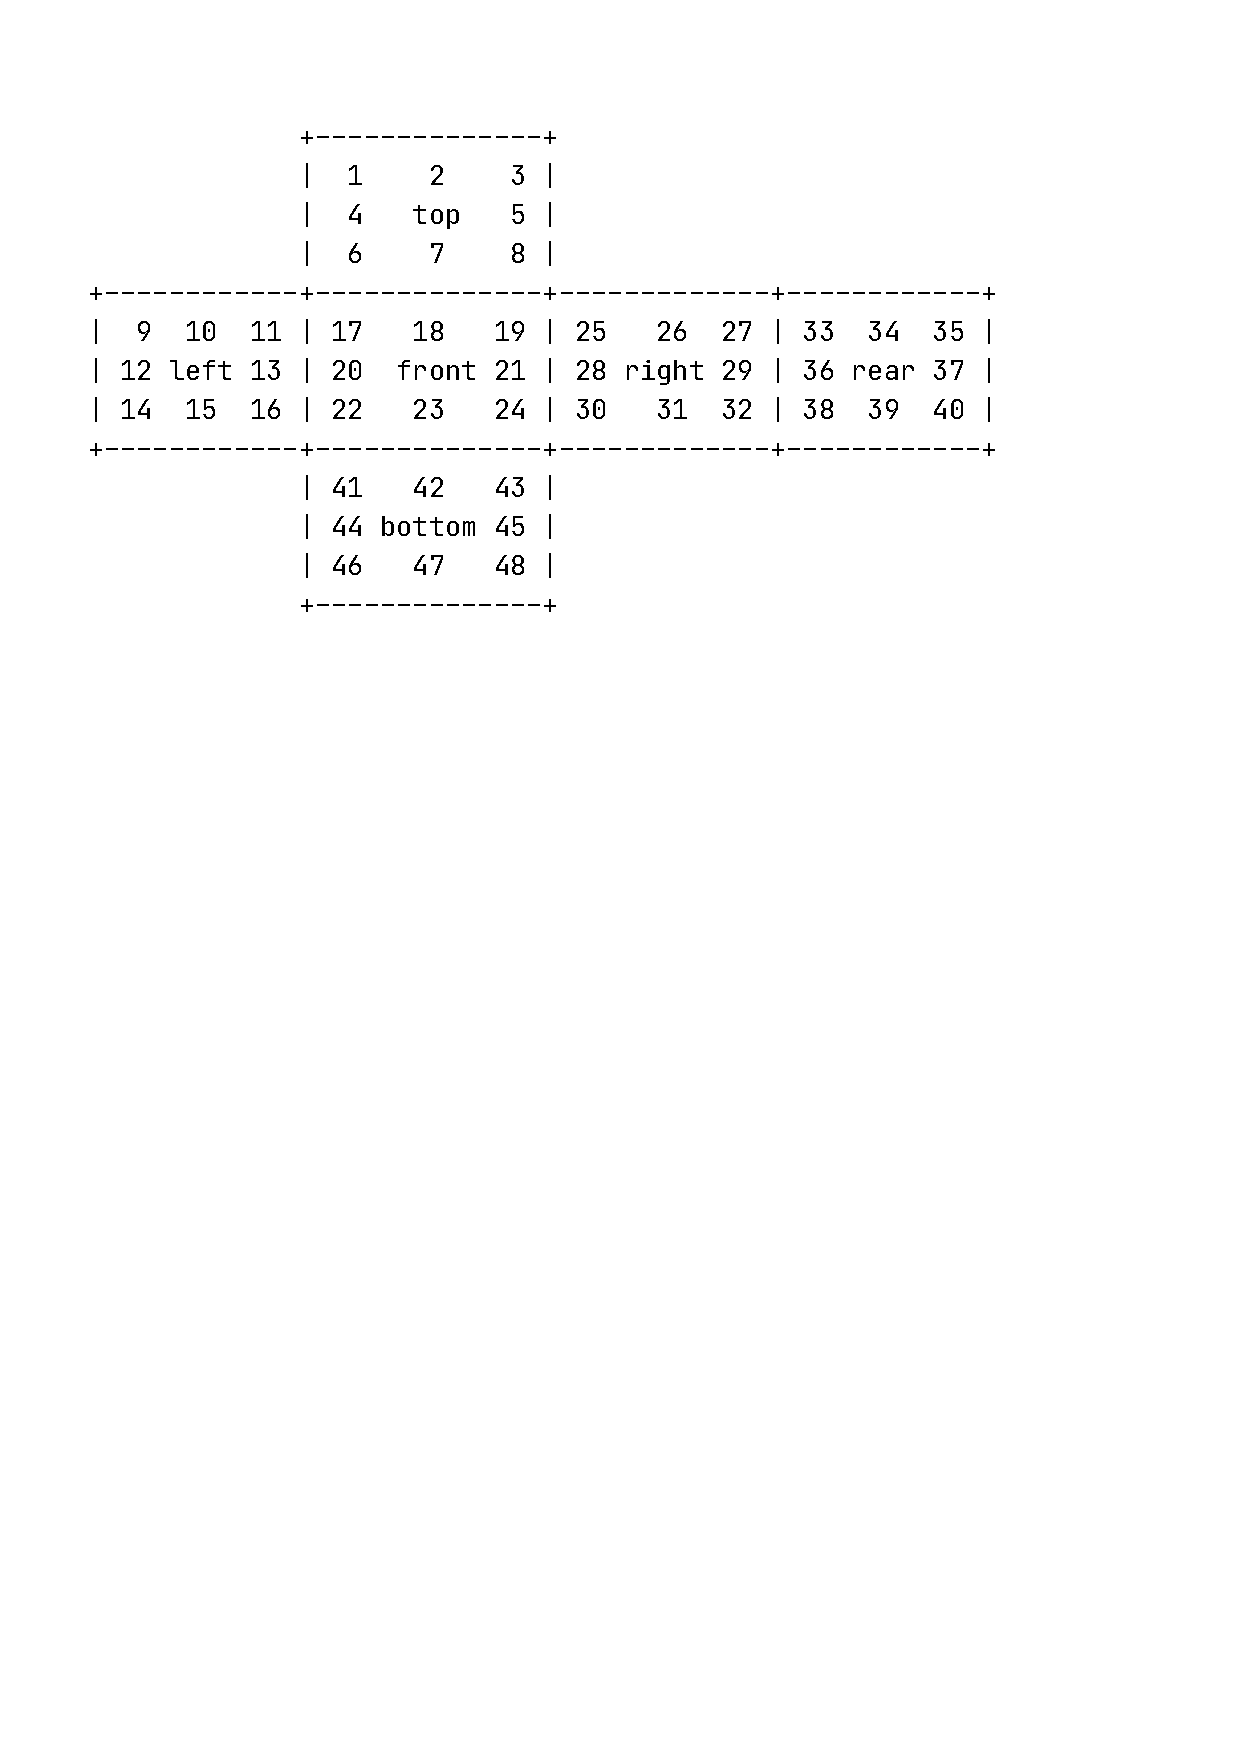
\includegraphics[scale=0.5]{images/display2d.pdf}
    \end{figure}
\end{frame}

\begin{frame}
    \frametitle{キューブ操作のシングマスター記法}

    \begin{figure}
        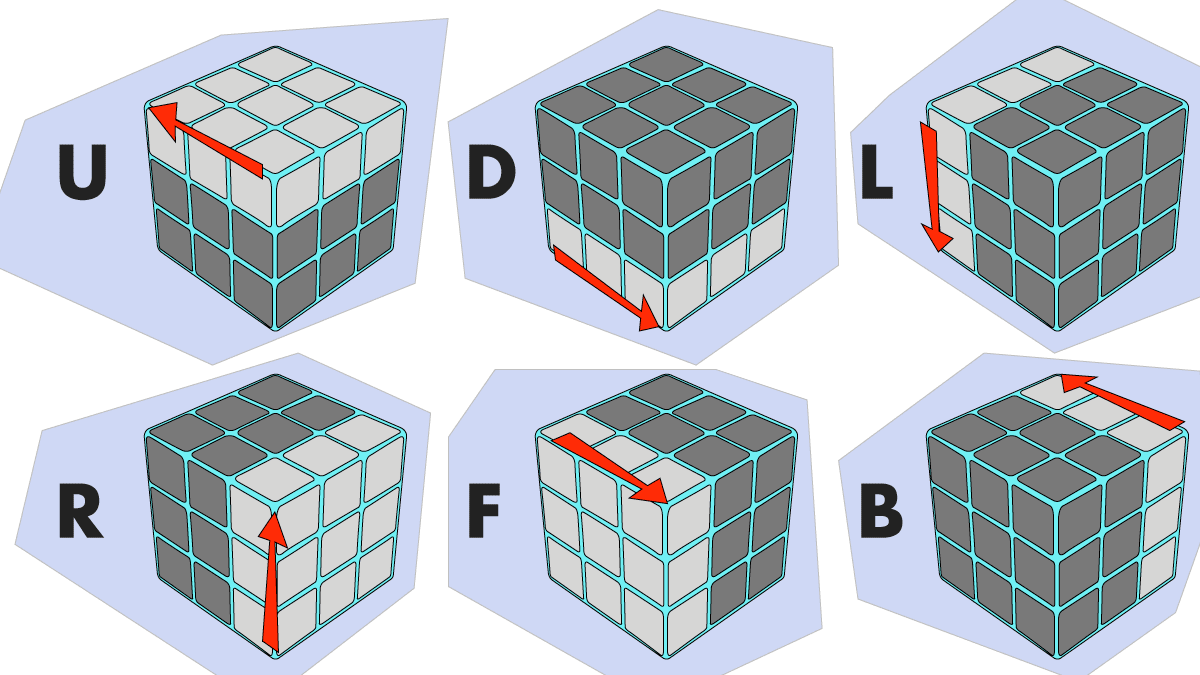
\includegraphics[scale=0.25]{images/singmaster.png}
    \end{figure}

    各面を時計回りに90度回転する操作を \(U, D, L, R, F, B\) と書きます。反時計回りは \(U'\) または \(U^{-1}\) と書きます。
\end{frame}

\begin{frame}
    \frametitle{ルービックキューブ群}

    \(X\) を小面48個の集合とします。キューブ操作は、\(X\) の置換写像であると考えることができます。\(X\) の置換全体の集合 \(S_X\) は群になります。これを \(X\) の対称群と呼びます。

    \bigskip

    \(S_X\) の中にはキューブ操作の組み合わせだけでは実現できないものもあります。例えば、3面体のひとつをルービックキューブから取り外して、小面のうち2つの色を逆に貼り替えてからルービックキューブに戻す、ということをします。これは小面集合 \(X\) の置換にはなっていますが、キューブ操作だけでは元の配置に戻すことができません。

    \bigskip

    基本操作 \(U, D, L, R, F, B\) で生成される \(S_X\) の部分群 \(G\) を、ルービックキューブ群と呼びます。

    \[
        G := \langle U, D, L, R, F, B \rangle \subset S_X
    \]
\end{frame}

\begin{frame}[fragile=singleslide]
    \frametitle{SageMath}

    \begin{figure}
        
\includegraphics[scale=0.25]{images/logo_sagemath+icon_oldstyle.png}
    \end{figure}

    SageMath は数学関連のソフトウェアを統合したものです。SageMath には、ルービックキューブ群を扱うプログラムが最初から組み込まれています。

    \bigskip

    \begin{minted}[autogobble]{sage}
        sage: rubik = CubeGroup()
        sage: rubik
    \end{minted}
    \begin{minted}[autogobble]{pycon}
        The Rubik's cube group with generators R,L,F,B,U,D
        in SymmetricGroup(48).
    \end{minted}
\end{frame}

\begin{frame}[fragile=singleslide]
    \frametitle{ルービックキューブのグラフィカル表示 (1)}

    \begin{minted}[autogobble]{sage}
        sage: rubik.display2d("")
        sage: rubik.plot_cube("")
        sage: rubik.plot3d_cube("")
    \end{minted}

    \begin{figure}
        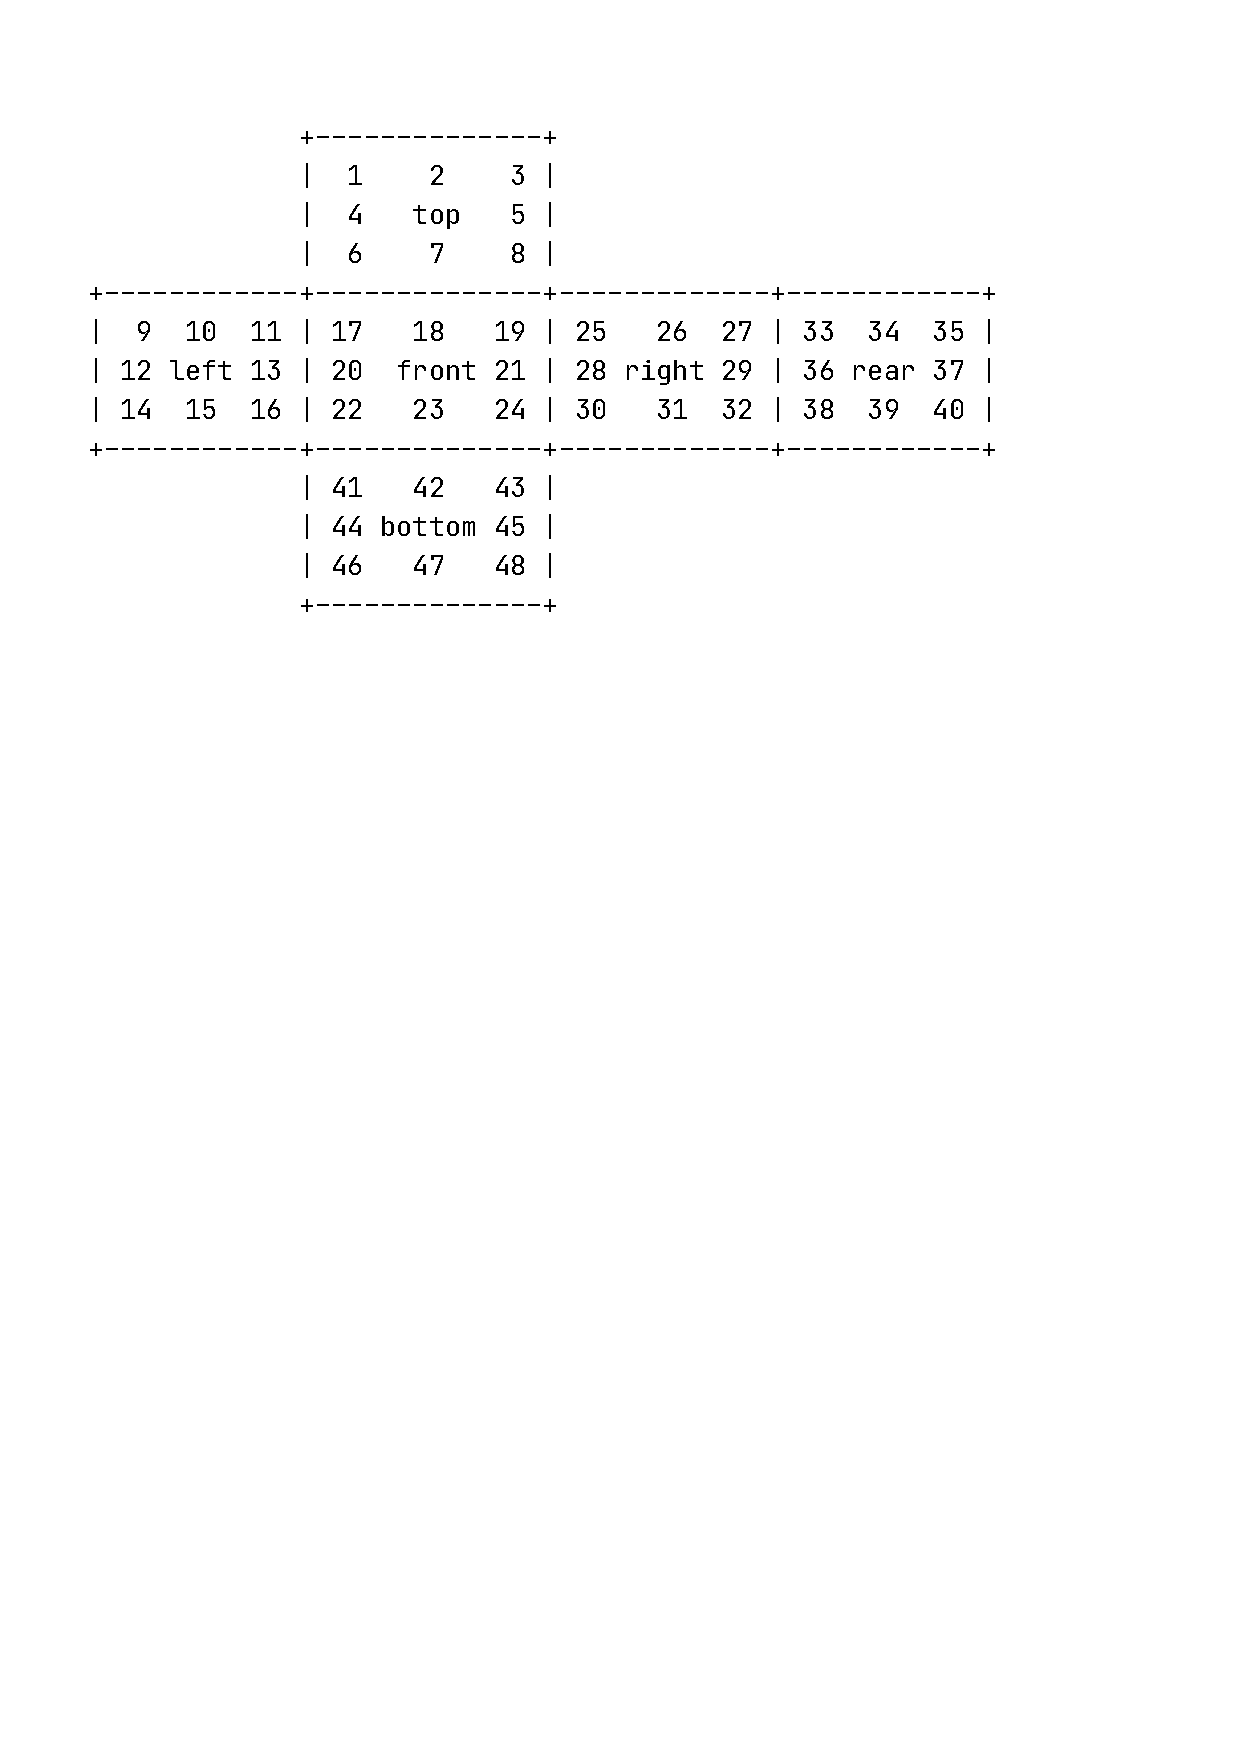
\includegraphics[scale=0.28]{images/display2d.pdf}
        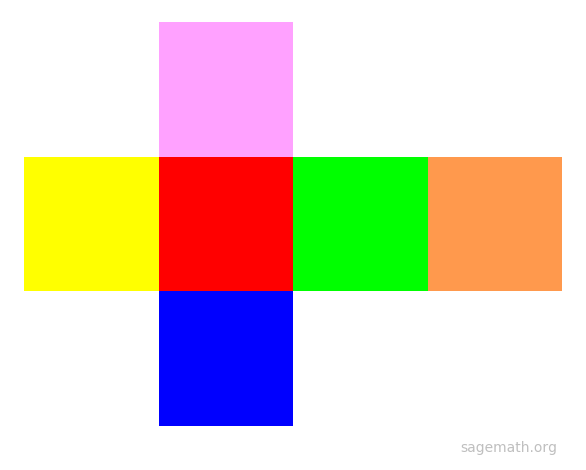
\includegraphics[scale=0.25]{images/plot_cube.png}
        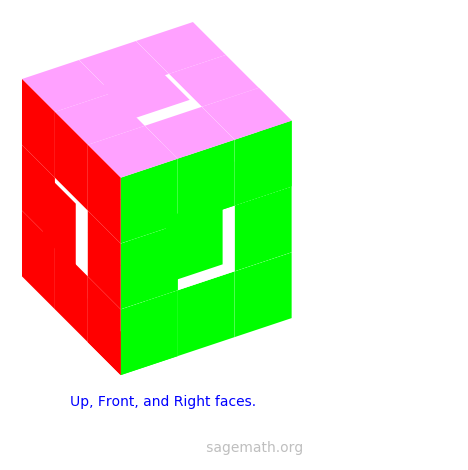
\includegraphics[scale=0.25]{images/plot3d_cube.png}
    \end{figure}
\end{frame}

\begin{frame}[fragile=singleslide]
    \frametitle{ルービックキューブのグラフィカル表示 (2)}

    \begin{minted}[autogobble]{sage}
        sage: rubik.plot_cube("R")
        sage: rubik.plot_cube("R U")
    \end{minted}

    \begin{figure}
        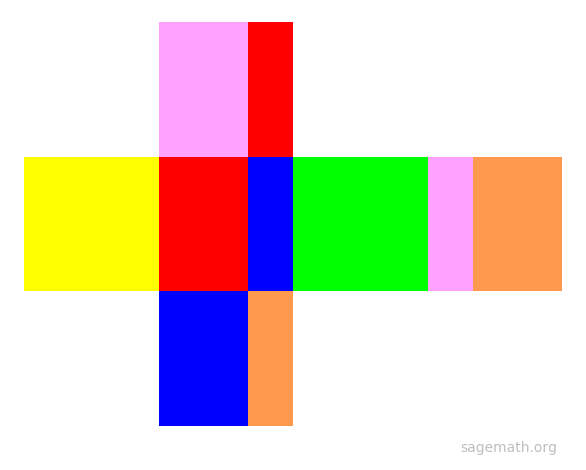
\includegraphics[scale=0.35]{images/plot_cube_R.png}
        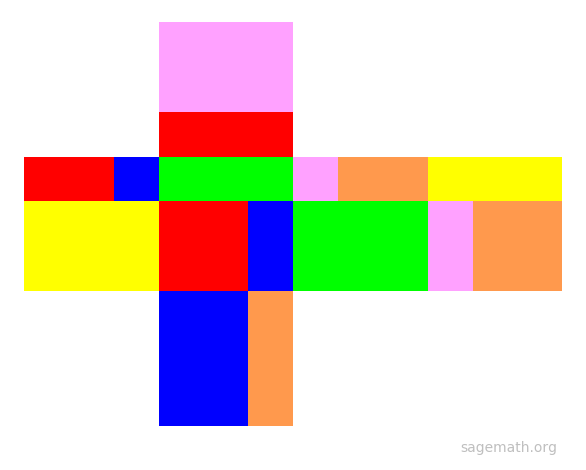
\includegraphics[scale=0.35]{images/plot_cube_RU.png}
    \end{figure}
\end{frame}

\begin{frame}[fragile=singleslide]
    \frametitle{ルービックキューブの操作 (1)}

    \begin{minted}[autogobble]{sage}
        sage: rubik.move("R")[0]
        (3,38,43,19)(5,36,45,21)(8,33,48,24)
        (25,27,32,30)(26,29,31,28)
    \end{minted}

    \bigskip

    操作 \(R\) は長さ 4 の巡回置換 5 個の積だと分かります。

    \bigskip

    \begin{minted}[autogobble]{sage}
        sage: rubik.move("R2")[0]
        (3,43)(5,45)(8,48)(19,38)(21,36)
        (24,33)(25,32)(26,31)(27,30)(28,29)
    \end{minted}

    \bigskip

    操作 \(R^2\) は長さ 2 の巡回置換 10 個の積だと分かります。
\end{frame}

\begin{frame}[fragile=singleslide]
    \frametitle{ルービックキューブの操作 (2)}

    \begin{minted}[autogobble]{sage}
        sage: rubik.move("R U")[0]
        (1,3,38,43,11,35,27,32,30,17,9,33,48,24,6)
        (2,5,36,45,21,7,4)(8,25,19)(10,34,26,29,31,28,18)
    \end{minted}

    \bigskip

    先ほどは長さ 2 や 4 の巡回置換でしたが、今回は長さ 7 や 11 の巡回置換が出てきているのが興味深いです。

    \bigskip

    \mintinline{sage}{(8,25,19)} に注目してみます。これは右上手前の小方体であり、操作 \(R U\) で元の位置に戻りますが、120 度回転しています。そのため、長さ 3 の巡回置換になっています。
\end{frame}

\begin{frame}[fragile=singleslide]
    \frametitle{ルービックキューブ群の位数}

    ルービックキューブ群は有限群です(有限集合の置換は有限個)。

    \bigskip

    その大きさがどれくらいなのか見てみます。

    \begin{minted}[autogobble]{sage}
        sage: rubik = CubeGroup()
        sage: rubik.order()
        43252003274489856000
        sage: rubik.order().factor()
        2^27 * 3^14 * 5^3 * 7^2 * 11
    \end{minted}

    \bigskip

    つまり、ルービックキューブで可能な配置は約 4325 京通りあることが分かります。
\end{frame}

\begin{frame}[fragile=singleslide]
    \frametitle{元の位数 (1)}

    \begin{definition}
        群の元 \(g\) について \(g^m = 1\) が成り立つような自然数 \(m\) で最小のものを、元 \(g\) の位数と呼びます。
    \end{definition}

    \begin{definition}
        ルービックキューブの特定の操作手順 \(g\) を \(m\) 回繰り返すと元の配置に戻るとき、その最小の \(m\) を \(g\) の位数と呼びます。
    \end{definition}

    操作 \(R\) は4回行えば元に戻るので \(R\) の位数は \(4\) です。

    \begin{minted}[autogobble]{sage}
        sage: rubik.move("R")[0].order()
        4
    \end{minted}
\end{frame}

\begin{frame}
    \frametitle{元の位数 (2)}

    \begin{theorem}
        有限群の元の位数は有限である。
    \end{theorem}

    これは、群の元 \(g\) に対して集合 \(\{ g^k \mid k \in \mathbb{Z}\}\) が部分群となることから分かります。

    \begin{theorem}
        ルービックキューブで特定の操作手順を何度も繰り返すと、必ず元の配置に戻る。
    \end{theorem}

    ルービックキューブで考えると成り立つかどうか分からない気がしますが、群論で考えるとわりと簡単に分かる、というのは興味深い点だと思います。
\end{frame}

\begin{frame}[fragile=singleslide]
    \frametitle{元の位数 (3)}

    では、操作 \(R U\) は何回やれば元に戻るのか?

    \begin{minted}[autogobble]{sage}
        sage: rubik.move("R U")[0].order()
        105
    \end{minted}

    \bigskip

    実際にやってみると、「え、これ本当に元に戻る・・・?」と不安になりますが、頑張って回すと本当に戻るのでちょっと感動。
\end{frame}

\begin{frame}[fragile=singleslide]
    \frametitle{元の位数 (4)}

    ルービックキューブ群には位数 \(1260\) の元があります。そのひとつが \(R U^2 D' B D'\) です。これより大きい位数の元はありません。

    \begin{minted}[autogobble]{sage}
        sage: rubik.move("R U2 D' B D'")[0].order()
        1260
    \end{minted}
\end{frame}

\begin{frame}[fragile=singleslide]
    \frametitle{操作手順の例:むすび}

    動く小面が少ない操作手順の例を挙げます。島内先生の本で「むすび」と呼んでいる手順です。操作は多いですが、結果を図で表示すると分かりやすいような気がします。

    \begin{minted}[autogobble]{sage}
        sage: rubik.plot_cube("R B L F U^2 F' L' B' R' U^2")
    \end{minted}

    \begin{figure}
        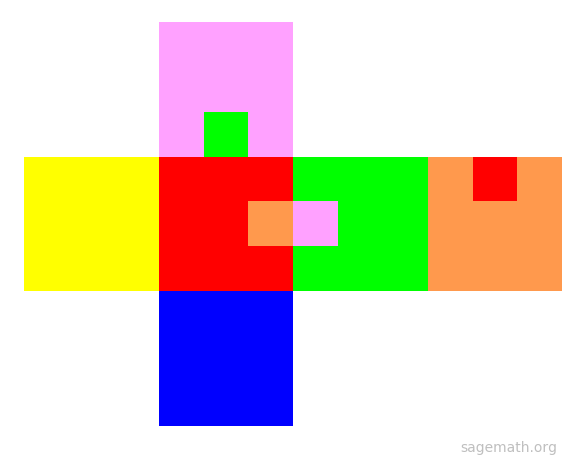
\includegraphics[scale=0.35]{images/plot_cube_musubi.png}
    \end{figure}
\end{frame}

\begin{frame}[fragile=singleslide]
    \frametitle{共役}

    群の元 \(g\) に対して(群の元 \(h\) を使って)\(h^{-1} g h\) の形の元を共役と呼びます。

    「むすび」の共役を考えると、別の場所の置換を作り出すことができます。

    \begin{minted}[autogobble]{sage}
        sage: rubik.plot_cube("R R B L F U^2 F' L' B' R' U^2 R'")
    \end{minted}

    \begin{figure}
        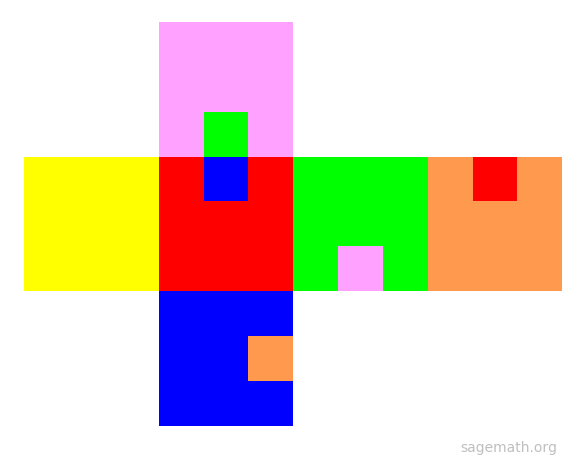
\includegraphics[scale=0.35]{images/plot_cube_musubi2.png}
    \end{figure}
\end{frame}

\begin{frame}
    \frametitle{参考文献}

    参考文献:

    \begin{itemize}
        \item \href{https://doc.sagemath.org/html/en/reference/groups/sage/groups/perm_gps/cubegroup.html}{Rubik's cube group functions - Sage Reference Manual}
        \item David Joyner、\href{https://www.amazon.co.jp/dp/4320019415/ref=nosim?tag=usamik-22}{群論の味わい -置換群で解き明かすルービックキューブと15パズル-}
        \item 島内剛一、\href{https://www.amazon.co.jp/dp/4535785376/ref=nosim?tag=usamik-22}{ルービック・キューブと数学パズル}
    \end{itemize}

    \bigskip

    David Joyner 先生が SageMath にルービックキューブ群を組み込んだようです。

    \bigskip

    島内先生の本には、ルービックキューブの様々な手順や、それを利用した解法が載っています。(残念ながら絶版ですが)
\end{frame}

\end{document}
